\documentclass[12pt,a4paper]{article}

% =============================================================
% SCSS / Student Scientific Conference Template
% Updated according to the new formatting requirements.
% Based on the original main.tex template.
% =============================================================

% -------------------- Page format --------------------
% A4; margins: top 30 mm, bottom 30 mm, left 25 mm, right 20 mm.
\usepackage[
    a4paper,
    left=25mm,
    right=20mm,
    top=30mm,
    bottom=30mm
]{geometry}

% -------------------- Font --------------------
% Font: Times New Roman, 12 pt.
% For exact Times New Roman, compile with XeLaTeX or LuaLaTeX.
% If compiled with pdfLaTeX, a Times-compatible font is used.
\usepackage{iftex}

\ifPDFTeX
    \usepackage[T1]{fontenc}
    \usepackage[utf8]{inputenc}
    \usepackage{newtxtext,newtxmath}
\else
    \usepackage{fontspec}
    \IfFontExistsTF{Times New Roman}
        {\setmainfont{Times New Roman}}
        {\setmainfont{Tinos}}
    \usepackage{newtxmath}
\fi

% -------------------- Packages --------------------
\usepackage[english]{babel}
\usepackage{setspace}
\usepackage{ragged2e}
\usepackage{titlesec}
\usepackage{graphicx}
\usepackage{indentfirst}
\usepackage{caption}
\usepackage{amsmath}
\usepackage{cite}
\usepackage{url}
\usepackage[hidelinks]{hyperref}

% -------------------- General text formatting --------------------
% Text: 12 pt, single spacing, justified.
\singlespacing
\AtBeginDocument{\justifying}
\setlength{\parindent}{1.25cm}
\setlength{\parskip}{0pt}

% -------------------- Paper metadata --------------------
% Fill in the fields below.

% Title: 14 pt, 1.5 line spacing, bold.
\newcommand{\PaperTitle}{\fontsize{14pt}{21pt}\selectfont\textbf{Template SCSS}}

% Authors and coordinator(s), centered on the same line.
% The last one or two names can be the scientific coordinator(s).
% The superscript 1 refers to affiliation 1 below.
\newcommand{\PaperAuthors}{Author1\textsuperscript{1}, Author2\textsuperscript{1}, Coordinator1\textsuperscript{1}, Coordinator2\textsuperscript{1}}

% Emails.
\newcommand{\PaperEmails}{email1@xyz.edu, email2@xyz.edu, coordinator1@xyz.edu, coordinator2@xyz.edu}

% Affiliation.
\newcommand{\PaperAffiliation}{\textsuperscript{1}Faculty of Automatic Control and Computer Science, National University of Science and Technology Politehnica Bucharest}

% Date.
\newcommand{\PaperDate}{\fontsize{12pt}{21pt}\selectfont\textbf{May 2026}}

% -------------------- Custom title block --------------------
% The title and author/coordinator line are centered.
\newcommand{\MakeSCSSTitle}{%
\begin{center}
    {\PaperTitle\par}
    \vspace{8pt}

    {\normalsize \PaperAuthors\par}
    \vspace{4pt}

    {\normalsize \textit{\PaperEmails}\par}
    \vspace{4pt}

    {\normalsize \PaperAffiliation\par}
    \vspace{4pt}

    {\normalsize \PaperDate\par}
\end{center}
\vspace{10pt}
}

% -------------------- Section formatting --------------------
% Chapters/sections: bold, left-aligned.
\titleformat{\section}
  {\normalfont\normalsize\bfseries}
  {\thesection.}{0.6em}{}

\titleformat{\subsection}
  {\normalfont\normalsize\bfseries}
  {\thesubsection.}{0.6em}{}

\titlespacing*{\section}{0pt}{12pt}{6pt}
\titlespacing*{\subsection}{0pt}{10pt}{4pt}

% -------------------- Abstract and keywords --------------------
\renewenvironment{abstract}{%
\begin{center}
    \normalsize\textbf{Abstract}
\end{center}
\itshape
}
{\par\normalfont\vspace{6pt}}

\newenvironment{keywords}
{\noindent\textbf{Keywords--}}
{\par\vspace{12pt}}

% -------------------- Figures and tables --------------------
% Figures:
% - numbered as Fig.1, Fig.2, etc.
% - caption below the figure
% - caption centered
% - caption font 11 pt
%
% Tables:
% - numbered as Table 1, Table 2, etc.
% - caption above the table
% - caption centered
% - caption font 11 pt
%
% If needed, indicate the source in square brackets:
% \caption{Example of a figure \cite{b1}}

\DeclareCaptionFont{captioneleven}{\fontsize{11pt}{13pt}\selectfont}
\DeclareCaptionLabelFormat{figlabel}{Fig.#2}
\DeclareCaptionLabelFormat{tablabel}{Table #2}

\captionsetup[figure]{
    font=captioneleven,
    labelformat=figlabel,
    labelsep=period,
    justification=centering,
    singlelinecheck=true,
    position=bottom
}

\captionsetup[table]{
    font=captioneleven,
    labelformat=tablabel,
    labelsep=period,
    justification=centering,
    singlelinecheck=true,
    position=top
}

% -------------------- Equations --------------------
% Use standard LaTeX equation settings.
% One blank line before and after displayed equations.
\setlength{\abovedisplayskip}{12pt plus 2pt minus 2pt}
\setlength{\belowdisplayskip}{12pt plus 2pt minus 2pt}
\setlength{\abovedisplayshortskip}{12pt plus 2pt minus 2pt}
\setlength{\belowdisplayshortskip}{12pt plus 2pt minus 2pt}

% -------------------- Bibliography title --------------------
\renewcommand{\refname}{References}

\begin{document}

\MakeSCSSTitle

\begin{abstract}
Lorem ipsum dolor sit amet, consectetur adipiscing elit. Praesent vel eros orci. Proin tincidunt lacinia tortor eu aliquet. Aenean nec consequat nisi, at eleifend nisl. Nam id dolor mi. Donec faucibus mauris et viverra maximus. Nullam nisi lectus, tincidunt a vehicula et, accumsan id libero. Fusce cursus lorem enim, in gravida nisi facilisis quis. Cras imperdiet mi at lorem sodales, tincidunt fermentum ipsum semper. Suspendisse potenti.
\end{abstract}

\begin{keywords}
Lorem, ipsum, dolor, sit, amet
\end{keywords}

\section{Introduction}

This section introduces the general context of the paper, the motivation for choosing the topic, and the relevance of the research problem. The introduction should briefly explain why the topic is important and how the paper is organized.

Lorem ipsum dolor sit amet, consectetur adipiscing elit. Praesent vel eros orci. Proin tincidunt lacinia tortor eu aliquet. Aenean nec consequat nisi, at eleifend nisl. Nam id dolor mi. Donec faucibus mauris et viverra maximus. Nullam nisi lectus, tincidunt a vehicula et, accumsan id libero.

\section{Problem Statement and Research Objectives}

This section clearly defines the analyzed problem and the research objectives.

\subsection{Analyzed Problem}

Describe the main problem addressed in the paper. Explain the context in which the problem appears, why it is relevant, and what limitations or challenges exist.

\subsection{Research Objectives}

Present the main objectives of the paper. The objectives should be clear, specific, and connected to the proposed solution and experimental evaluation.

\section{Relevant Scientific Context and State of the Art}

This section presents the scientific context relevant to the topic and discusses existing approaches from the literature.

\subsection{Relevant Scientific Context}

Explain the broader research area in which the paper is placed. Introduce the key concepts, technologies, or research directions related to the topic.

\subsection{State of the Art}

Present existing methods, systems, algorithms, tools, or studies related to the problem. References must be numbered and cited in the text using square brackets according to IEEE citation style. They must be introduced in the order in which they are used in the text, for example \cite{b1} and then \cite{b2}. Each bibliography entry must be cited at least once in the paper.

\subsection{Limitations of Existing Approaches}

Discuss the limitations of previous work and explain how these limitations motivate the proposed solution.

\section{Theoretical Aspects}

This section presents the theoretical concepts, models, definitions, algorithms, or mathematical foundations required to understand the proposed solution.

For formulas, use the standard LaTeX equation environment. Leave one blank line before and after displayed equations.

\begin{equation}
\label{eq:example}
S = \sum_{i=1}^{4} x_i \cdot y_i
\end{equation}

All numerical values appearing in the paper, including those included in tables, must be accompanied by the corresponding units of measurement where applicable, for example 10~m, 5~kg, 3~m/s\textsuperscript{2}, or 20~W.

\section{Proposed Solution}

This section describes the proposed method, system, architecture, algorithm, prototype, or workflow.

\subsection{Overview of the Proposed Solution}

Present the general idea of the solution and explain how it addresses the problem defined earlier.

\subsection{Architecture or Methodology}

Describe the architecture, components, workflow, algorithm, or methodology used in the proposed solution.

\subsection{Implementation Details}

Provide relevant implementation details, such as technologies, tools, libraries, datasets, or system components.

Figures must be inserted naturally in the text and scaled reasonably. Figure captions must be placed below the figure, centered, using 11 pt font. If applicable, the source must be indicated in square brackets in the caption.

Use Figure~\ref{fig:example} as a figure example.

\begin{figure}[htbp]
\centering
\IfFileExists{img/figure.png}{%
    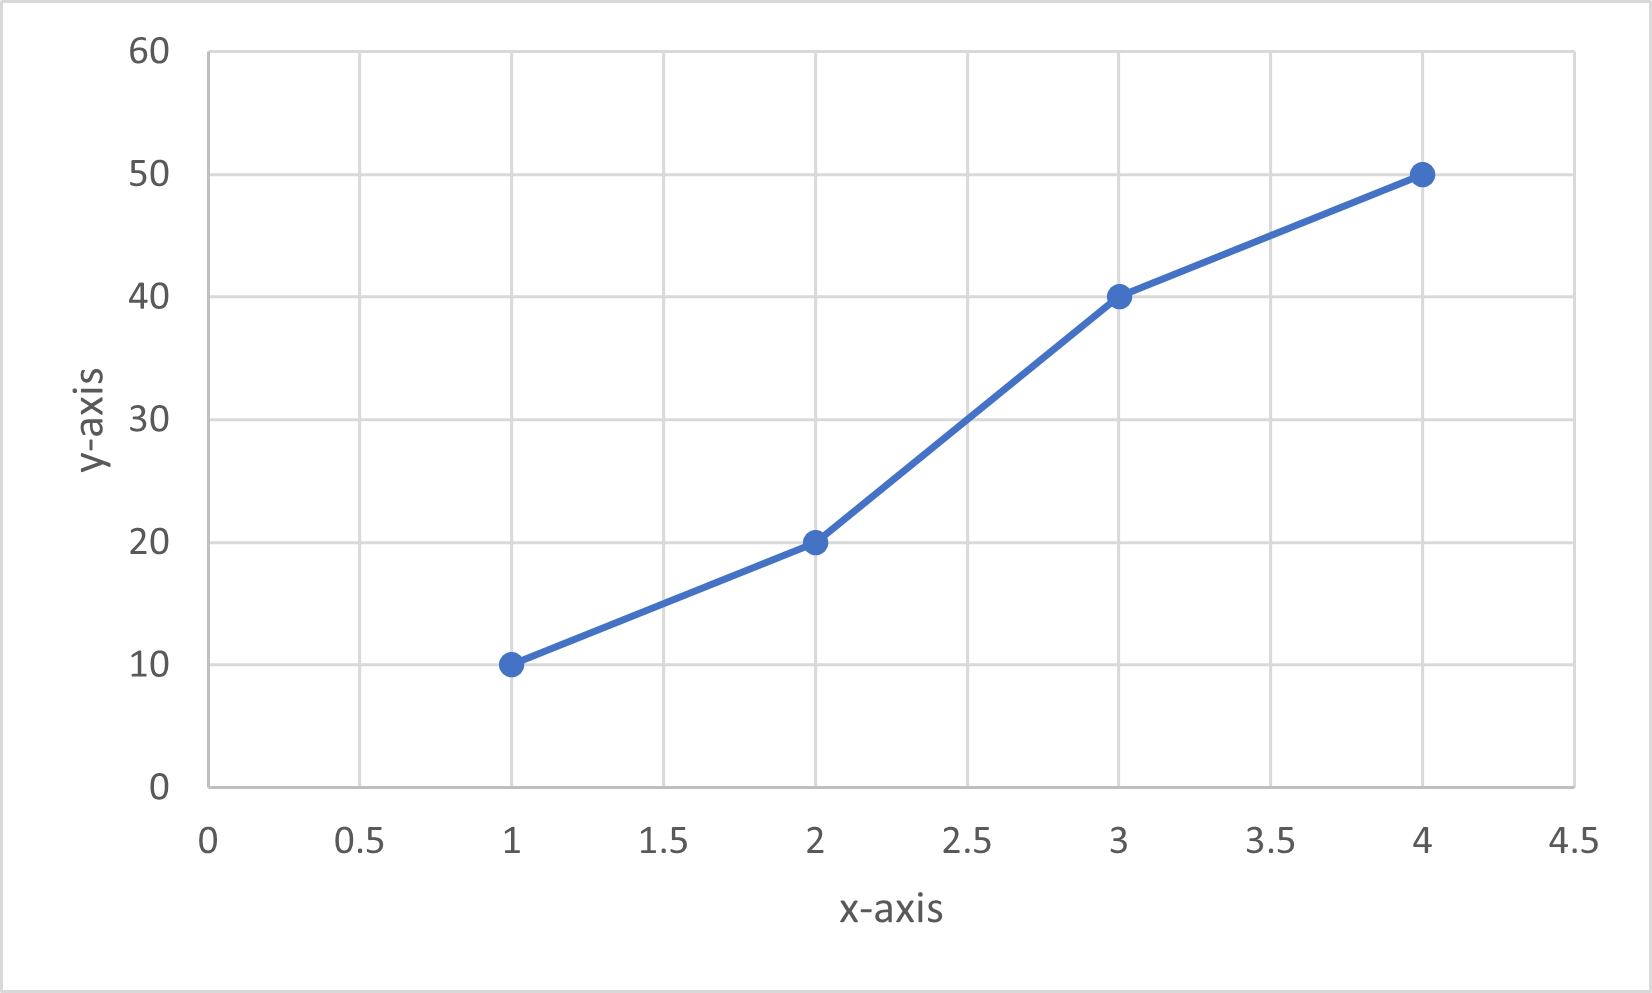
\includegraphics[width=0.75\linewidth]{img/figure.png}%
}{%
    \fbox{\rule{0pt}{35mm}\rule{0.75\linewidth}{0pt}}%
}
\caption{Example of a proposed solution diagram \cite{b1}}
\label{fig:example}
\end{figure}

\section{Experimental Realization}

This section describes how the experiments were designed and performed.

\subsection{Experimental Setup}

Describe the experimental environment, including hardware, software, operating system, tools, frameworks, and configuration details.

\subsection{Datasets and Input Data}

Present the datasets or input data used in the experiments. Include relevant characteristics such as size, number of samples, features, classes, or source, where applicable.

\subsection{Evaluation Metrics}

Define the metrics used to evaluate the proposed solution, such as accuracy, precision, recall, F1-score, execution time, memory usage, power consumption, or other relevant indicators.

\subsection{Experimental Scenarios}

Describe the experiments or test scenarios performed in order to validate the proposed solution.

Tables must be numbered and must have their title placed above the table, centered, using 11 pt font.

Use Table~\ref{tab:example} as a table example.

\begin{table}[htbp]
\centering
\caption{Example of experimental measurements \cite{b2}}
\label{tab:example}
\begin{tabular}{c c c}
 \hline
 \textbf{Experiment} & \textbf{Execution time [s]} & \textbf{Power [W]} \\
 \hline
 E1 & 10 & 45 \\
 E2 & 20 & 48 \\
 E3 & 40 & 51 \\
 E4 & 50 & 53 \\
 \hline
\end{tabular}
\end{table}

\section{Results Interpretation}

This section interprets the obtained experimental results and connects them to the research objectives.

\subsection{Analysis of Results}

Explain the meaning of the obtained results. Highlight the most important observations and trends.

\subsection{Comparison with the Objectives}

Discuss whether the proposed solution achieved the research objectives defined earlier.

\subsection{Limitations and Discussion}

Mention the limitations of the current work, possible sources of error, and aspects that could be improved in future work.

\section{Conclusions}

This section summarizes the analyzed problem, the proposed solution, the main results, and the contribution of the paper. Future research directions may also be mentioned.

\begin{thebibliography}{99}
\setlength{\itemsep}{0pt}

\bibitem{b1} G. Eason, B. Noble, and I. N. Sneddon, ``On certain integrals of Lipschitz-Hankel type involving products of Bessel functions,'' \emph{Phil. Trans. Roy. Soc. London}, vol. A247, pp. 529--551, April 1955.

\bibitem{b2} J. Clerk Maxwell, \emph{A Treatise on Electricity and Magnetism}, 3rd ed., vol. 2. Oxford: Clarendon, 1892, pp. 68--73.

\end{thebibliography}

\end{document}